\documentclass{beamer}
\usepackage{panyan_beamer}
\usepackage[normalem]{ulem}
\usetheme{Madrid}
\usecolortheme{default}
\title{Zeroth-Order Online Convex Optimization}
\author{Yan Pan}
\institute{Carnegie Mellon University}
\date{\today}

\begin{document}
\frame{\titlepage}

\begin{frame}
    \frametitle{Convex Optimization}
    \begin{itemize}
        \item A set $\Dc$ is convex if for every $x, y \in \Dc$, $0 \le \lambda \le 1$, we have
        \[
            \lambda x + (1 - \lambda) y \in \Dc.
        \]
        \item A function $f : \Dc \to \R$ is convex if $\Dc$ is convex and for every $x, y \in \Dc$, $0 \le \lambda \le 1$,
        \[
            f(\lambda x + (1 - \lambda) y) \le \lambda f(x) + (1 - \lambda) f(y)
        \]
        \begin{center}
            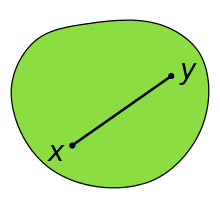
\includegraphics[width=0.2\textwidth]{convex_set.png}
            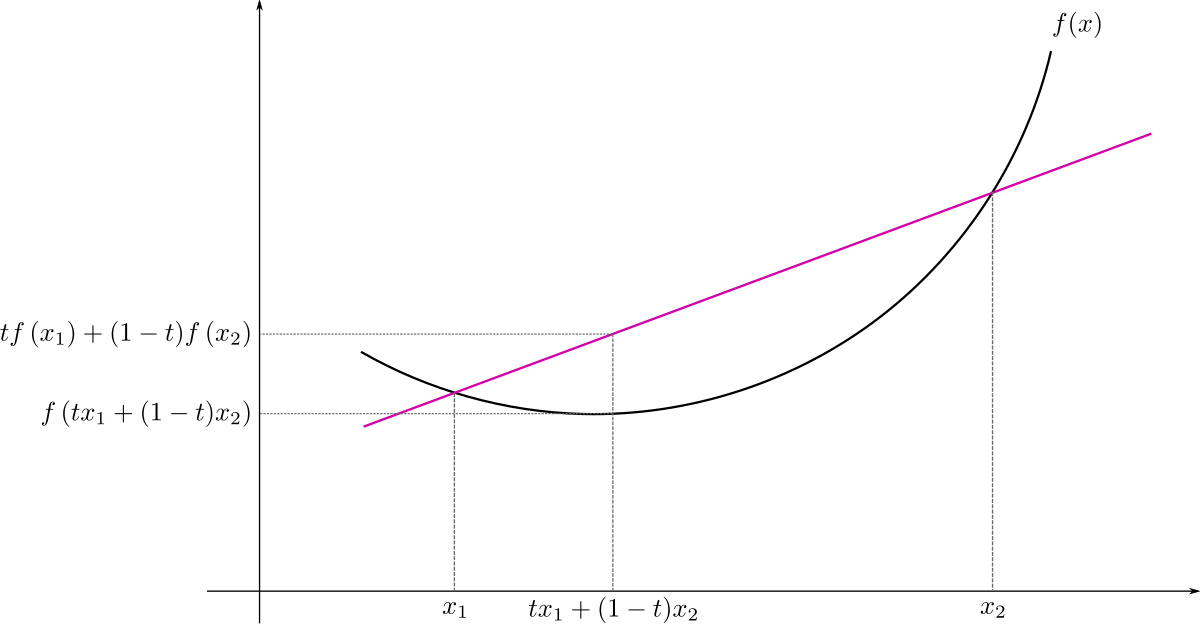
\includegraphics[width=0.35\textwidth]{convex_function.png}
        \end{center}
        \item If $\nabla f(x^*) = 0$, then $x^*$ is the only global/local minima of $f$.
    \end{itemize}
\end{frame}

\begin{frame}
    \frametitle{Examples of Convex Functions}
    \begin{itemize}
        \item Most classical machine learning models (e.g. linear regression, logistic regression, SVM, kernel methods)
        \item Most loss functions (e.g. mean squared loss, cross-entropy loss)
        \item \sout{Neural networks (unfortunately they are not convex, but somehow many convex optimization algorithms still work; this is another interesting field of research)}
    \end{itemize}
\end{frame}

\begin{frame}
    \frametitle{(Stochastic) Gradient Descent}
    \begin{itemize}
        \item At every timestep $t$, update
        \[
            x_{t+1} = x_t - \eta g_t.
        \]
        \item In \textbf{gradient descent}, $g_t = \nabla f(x_t)$.
        \item In \textbf{stochastic gradient descent}, $g_t$ is a random vector, such that $\E[g_t] = \nabla f(x_t)$, and $\E[\norm{g_t}^2] \le G$ for some constant $G$.
        \item If the constraint set $\Dc$ is a closed and bounded convex set, we can do \textbf{projected gradient descent}, where we project $x_{t+1}$ back to $\Dc$ if it is ``out of bound'',
        \[
            x_{t+1} = P_\Dc(x_t - \eta g_t).
        \]
    \end{itemize}
\end{frame}

\begin{frame}
    \frametitle{Convergence of SGD}
    \begin{itemize}
        \item It is not hard to show that gradient descent converges.
        \item We need to assume that $f$ is convex and $\norm{\nabla^2 f(x)} \le L$ (``$L$-smooth'').
    \end{itemize}
\end{frame}

\begin{frame}
    \frametitle{Convergence of Gradient Descent}
    \begin{itemize}
        \item If $f$ is convex, then
        \[
            f(y) \ge f(x) + \angles{\nabla f(x), y - x}.
        \]
        \item Plugging into $y = x^*$, $x = x_t$, we have
        \begin{align*}
            f(x^*) &\ge f(x_t) + \angles{\nabla f(x_t), x^* - x_t}\\
            &= f(x_t) + \frac{1}{\eta}\angles{x_t - x_{t+1}, x^* - x_t}.
        \end{align*}
        \item By ``law of cosines'', we get an interesting formula
        \begin{align*}
            f(x_t)
            &\le f(x^*) + \frac{1}{2\eta}\parens*{\norm{x^* - x_t}^2 - \norm{x^* - x_{t+1}}^2 + \norm{x_t - x_{t+1}}^2}\\
            &\le f(x^*) + \frac{1}{2\eta}\parens*{\norm{x^* - x_t}^2 - \norm{x^* - x_{t+1}}^2 + \eta^2 \norm{g_t}^2}.
        \end{align*}
    \end{itemize}
\end{frame}

\begin{frame}
    \frametitle{Convergence of Gradient Descent}
    \begin{itemize}
        \item Then, summing up from $t=1,\dots,T$, we have
        \[
            \frac{1}{T}\sum_{t=1}^T f(x_t) \le f(x^*) + \frac{1}{2\eta}\parens*{\norm{x^* - x_0}^2 + \eta^2 \sum_{t=1}^T \norm{g_t}^2}
        \]
        \item We just need to bound $\norm{g_t}^2$!
    \end{itemize}
\end{frame}

\begin{frame}
    \frametitle{Convergence of Gradient Descent}
    \begin{itemize}
        \item For gradient descent, if $f$ is $L$-smooth, then by Taylor's theorem,
        \[
            f(y) \le f(x) + \angles{\nabla f(x), y - x} + \frac{L}{2} \norm{y - x}^2.
        \]
        \item Plugging into $y = x_{t+1}$ and $x = x_t$, we have
        \begin{align*}
            f(x_{t+1})
            &\le f(x_t) + \angles{\nabla f(x_t), x_{t+1} - x_t} + \frac{L}{2} \norm{x_{t+1} - x_t}^2\\
            &\le f(x_t) - \eta \norm{\nabla f(x_t)}^2 + \frac{L}{2}\eta^2 \norm{\nabla f(x_t)}^2.
        \end{align*}
        \item Choosing $\eta = \frac{1}{L}$, we have
        \[
            \norm{\nabla f(x_t)}^2 \le \frac{2}{\eta}(f(x_t) - f(x_{t+1}))
        \]
        so the sum is $O(1/\eta)$.
        \item The average loss is at most $O(1/T)$.
    \end{itemize}
\end{frame}
\begin{frame}
    \frametitle{Convergence Rate of Gradient Descent}
    \begin{itemize}
        \item For SGD, we just bound $\norm{g_t}^2$ by the variance, so sum is $O(T)$.
        \item We can pick $\eta = O(1/\sqrt{T})$ in this case, so the average loss is at most $O(1/\sqrt{T})$.
    \end{itemize}
\end{frame}

\begin{frame}
    \frametitle{Online Convex Optimization}
    \begin{itemize}
        \item Instead of a single objective function, a sequence of functions $f_1, f_2, \dots$ is given.
        \item Need to pick a point $x_t$ before knowing anything about $f_t$.
        \item Try to minimize the regret compared to the minima $x^*$ of the sum
        \[
            R_T := \sum_{t=1}^T f_t(x_t) - \min_{x^* \in \Dc} \sum_{t=1}^T f_t(x^*).
        \]
        \item Goal is to make $\lim_{T \to \infty} \frac{R_T}{T} \to 0$, so we have vanishing average regret.
    \end{itemize}
\end{frame}

\begin{frame}
    \frametitle{Examples of Online Optimization}
    \begin{itemize}
        \item \textbf{(Mini-batch) stochastic gradient descent}: At every epoch, sample a batch from the dataset, and optimize the loss on the batch. This is the most widely used optimization algorithm in machine learning.
        \item \textbf{Non-convex optimization}: In empirical risk minimization, to minimize $f(w) = \sum_{i=1}^N \ell(h(w, x_i), y_i)$, with the model $h$ non-convex and loss $\ell$ convex, we can equivalently solve the following online convex optimization problem
        \[
            f_t(w) = \frac{1}{N} \sum_{i=1}^N \ell(h(w_t, x_i) + \angles{\nabla_w h(w_t, x_i), w - w_t}, y_i).
        \]
    \end{itemize}
\end{frame}

\begin{frame}
    \frametitle{Examples of Online Optimization}
    \begin{itemize}
        \item \textbf{Multi-armed bandits}: There are $d$ machines and you can pick which one to play. After you play, you can observe the full reward vector $\ell_t$. We can maintain a probability distribution $p_t$ and define $f_t(p_t) = -\angles{\ell_t, p_t}$. Then, we can optimize using projected gradient descent.
        \item \textbf{Reinforcement learning}: The environment changes when the player makes an action. The objective function (``value function'') is dependent on the current state and the player's action.
    \end{itemize}
\end{frame}

\begin{frame}
    \frametitle{Gradient Descent Still Works}
    \begin{itemize}
        \item This problem seems hard, since we don't know anything about functions in the future.
        \item Typically, there is no guarantee that the functions are similar.
        \item Surprisingly, gradient descent can still minimize the regret, even if we use a different function for every update step!
        \item This is because the baseline is the minimizer of the sum $\min_{x^* \in \Dc}\sum_{t=1}^T f_t(x^*)$, and not the minimizers of each function.
    \end{itemize}
\end{frame}

\begin{frame}
    \frametitle{Proof of Gradient Descent Convergence}
    \begin{itemize}
        \item The proof is pretty much the same as the stochastic gradient case.
        \item We assume $f_t$ to be Lipschitz, that is for every $x,y \in \Dc$,
        \[
            \abs{f(x) - f(y)} \le L\norm{x-y}
        \]
        which bounds the gradient $\norm{\nabla f(x)} \le L$.
        \item The regret is $O(\sqrt{T})$, so the average regret is vanishing~\citep{zinkevich2003online}.
    \end{itemize}
\end{frame}


\begin{frame}
    \frametitle{Zeroth-Order Online Convex Optimization}
    \begin{itemize}
        \item At every timestep $t$, instead of $\nabla f_t(x_t)$, we can only observe $f_t(x_t)$.
        \item This is natural in scenarios where gradient is hard to obtain, or the objective function is not differentiable.
        \item Can we still use our favorite gradient-based methods?
    \end{itemize}
\end{frame}

\begin{frame}
    \frametitle{Revisiting an Example}
    \begin{itemize}
        \item A company wants to decide how much money to spend on advertising their products in $d$ channels.
        \item The objective function is the profit, which is changing rapidly over time, and in general there is no guarantee about how it will change.
        \item The company definitely cannot know anything about the future, and they need to choose the allocations before observing the profit.
        \item The gradient is hard to obtain in this case --- they don't know what the objective function is. They only know their profits.
    \end{itemize}
\end{frame}

\begin{frame}
    \frametitle{An Offline Solution}
    \begin{itemize}
        \item We may try to approximate $\nabla f(x)$ by
        \[
            \angles{\nabla f(x), u} = \lim_{\delta \to 0} \frac{f(x + \delta u) - f(x)}{\delta}.
        \]
        \item Pick a sufficiently small $\delta$, so when $f$ is Lipschitz, this will be a good approximation of the partial derivatives.
        \item In $\R^d$, we need to approximate $d$ times to estimate the gradient.
        \item But in the online setting, we can only observe the value of $f_t$ at one point! Once we observe the value, the objective function changes to $f_{t+1}$, and we cannot get more information about $f_t$.
    \end{itemize}
\end{frame}

\begin{frame}
    \frametitle{Solution of~\cite{flaxman2005online}}
    \begin{itemize}
        \item What if we can sample a unit random vector?
        \item Key idea: Use Stoke's theorem to approximate the stochastic gradient.
        \[
            \nabla f(x) \approx \E_{u \sim \Sc}\bracks*{\frac{d}{\delta} f(x + \delta u) u} = \E_{u \sim \Sc}\bracks*{\frac{d}{\delta} (f(x + \delta u) - f(x)) u}
        \]
        \item We only need the function value at one point $f(x + \delta v)$ to approximate the stochastic gradient!
    \end{itemize}
\end{frame}
\begin{frame}
    \frametitle{Solution of~\cite{flaxman2005online}}
    \begin{itemize}
        \item Formally, let $\Sc$ be the unit sphere in $\R^d$, and $\Bc$ be the unit ball in $\R^d$.
        \item By Stoke's theorem
        \[
            \nabla \int_{\delta \Bc} f(x + v)~dv = \int_{\delta \Sc} f(x + u) \frac{u}{\norm{u}}~du.
        \]
        \item Then, since $\vol(\Bc) = d\vol(\Sc)$, we have
        \[
            \E_{u \sim \Sc}\bracks*{\frac{d}{\delta} f(x + \delta u) u} = 
            \nabla \wh{f}(x)
        \]
        where
        \[
            \wh{f}(x) = \E_{v \sim \Bc}[f(x + \delta v)].
        \]
    \end{itemize}
\end{frame}
\begin{frame}
    \frametitle{Solution of~\cite{flaxman2005online}}
    \begin{itemize}
        \item If we sample $v \sim S$, then $\frac{d}{\delta} f(x + \delta v)v$ is a stochastic gradient of $\wh{f}$ at $x$, which we can use to do stochastic gradient descent.
        \item $\wh{f}$ is an ``average'' of $f$ in a neighborhood of radius $\delta$, so when $\delta$ is small and $f$ is Lipschitz, the difference between $f$ and $\wh{f}$ is small.
        \item Algorithm: At every timestep, sample $u_t \sim \Sc$, and update using
        \[
            x_{t+1} = P_\Dc\parens*{x_t - \eta \frac{\delta}{d} f_t(x_t + \delta u_t)u_t}.
        \]
    \end{itemize}
\end{frame}

\begin{frame}
    \frametitle{Bounding the Regret}
    \begin{itemize}
        \item We can bound $\norm{g_t}^2 \le \frac{d}{\delta} \max_{x \in \Dc} \abs{f_t(x)}$.
        \item The standard online gradient descent proof gives us a bound on the regret of $\wh{f}_t$ as $O(\frac{\sqrt{T}}{\delta})$.
        \item However, this is a bound on the regret of $\wh{f}_t$! We know that if each $f_t$ is Lipschitz, then there is an additional error of
        \[
            \sum_{t=1}^T f_t(x_t) - \sum_{t=1}^T \wh{f}_t(x_t) \le O(\delta T)
        \]
        \item Choosing $\delta = O(T^{-1/4})$ gives us a regret of $O(T^{3/4})$.
    \end{itemize}
\end{frame}

\begin{frame}
    \frametitle{Extensions of the Setting}
    \begin{itemize}
        \item There are various extensions of this ``bandit'' setting in online convex optimization.
        \item Better algorithms exist if additional assumptions are made.
    \end{itemize}
\end{frame}

\begin{frame}
    \frametitle{Two-Point Estimates~\citep{agarwal2010optimal}}
    \begin{itemize}
        \item When we have two points as feedback, similarly we can estimate the gradient by
        \[
            \nabla f(x) \approx \E_{u \sim \Sc} \bracks*{\frac{d}{2\delta}(f(x + \delta u) - f(x - \delta u)) u}.
        \]
        \item When $f$ is Lipschitz, $\abs{f(x + \delta u) - f(x - \delta u)} \le 2\delta$, so we removed the $\delta^{-1}$ factor in the bound of $\norm{g_t}$!
        \item Then, we can choose $\delta = O(\frac{1}{\sqrt{T}})$, so regret is bounded by $O(\sqrt{T})$, which asymptotically is as good as when we have the gradient!
    \end{itemize}
\end{frame}

\begin{frame}
    \frametitle{Smooth Objective Functions~\citep{saha2011improved}}
    \begin{itemize}
        \item What if we sample from other than a sphere?
        \item For a positive semidefinite matrix $A$, we can also approximate by
        \[
            \nabla \wh{f}(x) = \frac{d}{\delta}f(x + \delta A u)A^{-1}u
        \]
        where $u \sim \Sc$ and
        \[
            \wh{f}(x) = \E_{u \sim \Bc}[f(x + \delta Au)].
        \]
        \item \cite{saha2011improved} improve the regret to $O(T^{2/3})$ for smooth functions by finding a sequence of $A_t$ from a self-concordant barrier function using an interior point method.
    \end{itemize}
\end{frame}

\begin{frame}
    \frametitle{Application in Concave Games~\citep{bravo2018bandit}}
    \begin{itemize}
        \item Suppose we have a repeated game, where each players have a concave utility function $u_i$.
        \item The players can only optimize their action $x_i$, but they cannot control the action of other players $x_{-i}$.
        \item We can define $f_t(x_{t,i}) = u_i(x_{t,i}, x_{t,-i})$, then this becomes an online optimization problem.
        \item The individual players can use the algorithm by~\cite{flaxman2005online} if they only receive their utility as feedback.
        \item \cite{bravo2018bandit} shows that the game converges to a Nash equilibrium if the players use this strategy.
    \end{itemize}
\end{frame}

\bibliography{references}
\bibliographystyle{apalike}
\end{document}
